\documentclass[xcolor={dvipsnames}, handout]{beamer}

\usepackage{amsmath,amsfonts,amssymb,pxfonts,eulervm,xspace}
\usepackage{mathrsfs} % math script fonts
\usepackage{tikz}
\usetikzlibrary{calc} %boxes
\newcommand{\tikzmark}[1]{\tikz[overlay,remember picture] \node (#1) {};}
\usetikzlibrary{cd} % commutative diagrams
\usepackage{subcaption} % subfigure float captioning

\usepackage{tabularx}
\usepackage{multirow}
\usepackage{graphicx}
\usepackage{appendixnumberbeamer} 

\usepackage{notation} % move this later

\graphicspath{.figures/}

\usepackage[backend=bibtex, style=numeric-comp, doi=false,isbn=false,url=false, giveninits=true]{biblatex}
\bibliography{../draft/glasslab_viz.bib}

\usetheme{ccnycrest}

\newenvironment{changemargin}[2]{%
\begin{list}{}{%
\setlength{\topsep}{0pt}%
\setlength{\leftmargin}{#1}%
\setlength{\rightmargin}{#2}%
\setlength{\listparindent}{\parindent}%
\setlength{\itemindent}{\parindent}%
\setleng{}th{\parsep}{\parskip}%
}%
\item[]}{\end{list}}

\begin{document}

\title{Topological Equivariant Artist Model}

\begin{frame}
	\titlepage
    Hannah Aizenman\\
    Advisor: Dr. Michael Grossberg \\
    Committee: Dr. Robert Haralick, Dr. Lev Manovich, Dr. Huy Vo\\
    External Member: Dr. Marcus Hanwell
\end{frame}

\section{Introduction}

\begin{frame}{Visualizations are structure preserving maps}
    \begin{figure}
        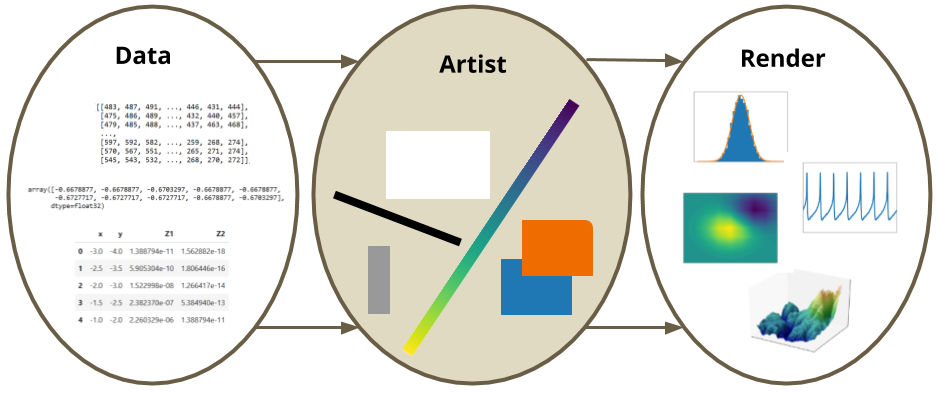
\includegraphics[width=1\linewidth]{figures/intro/dar.png}
    \end{figure}
    The aim of this work is to rearchitecture Matplotlib
    \pause 
    to take advantage of developments in software design, data structures, and visualization
    \pause
    to improve consistency, reusability, and discoverability,
    \pause
    so domain specific tool developers can build structure preserving visualization tools.
\end{frame}

\begin{frame}{Visualization component constraints}
    \begin{description}
        \item[equivariance] properties of data and visual encoding match
        \item[continuity] connectivity of data and visual encoding match
        \item[composibility] structure preserved by individual components is preserved in combined components
    \end{description}
\end{frame}

\subsection{Background}
\begin{frame}{Tools are tuned to the continuity of the date \cite{HeerSoftware2006,toryRethinkingVisualizationHighlevel2004}}
    \begin{columns}
        \column{0.33\textwidth}
        \begin{figure}
            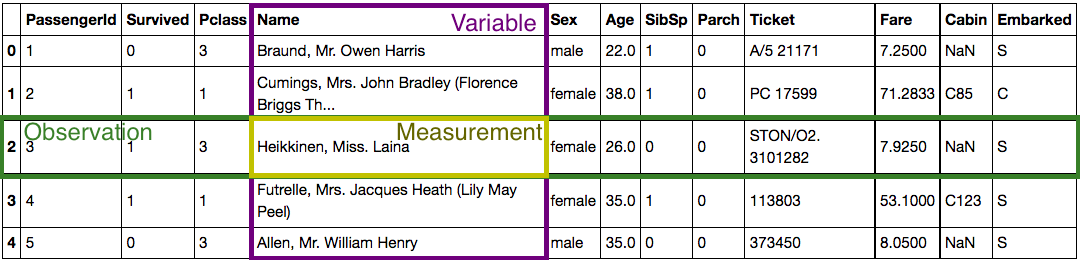
\includegraphics[width=1\textwidth]{figures/intro/data_formatting.png}
            \caption{Based on fig~2.5 in Munzner's VAD\cite{VisualizationAnalysisDesign}}
        \end{figure}
    
        \begin{enumerate}
            \item ggplot\cite{wickhamGgplot2ElegantGraphics2016a}
            \item protovis\cite{bostockProtoviz2009}, D3 \cite{bostockDataDrivenDocuments2011}
            \item vega\cite{satyanarayanDeclarativeInteractionDesign2014}, altair\cite{vanderplasAltairInteractiveStatistical2018}
        \end{enumerate}
        \pause
        \column{0.33\textwidth}
        \begin{figure}
            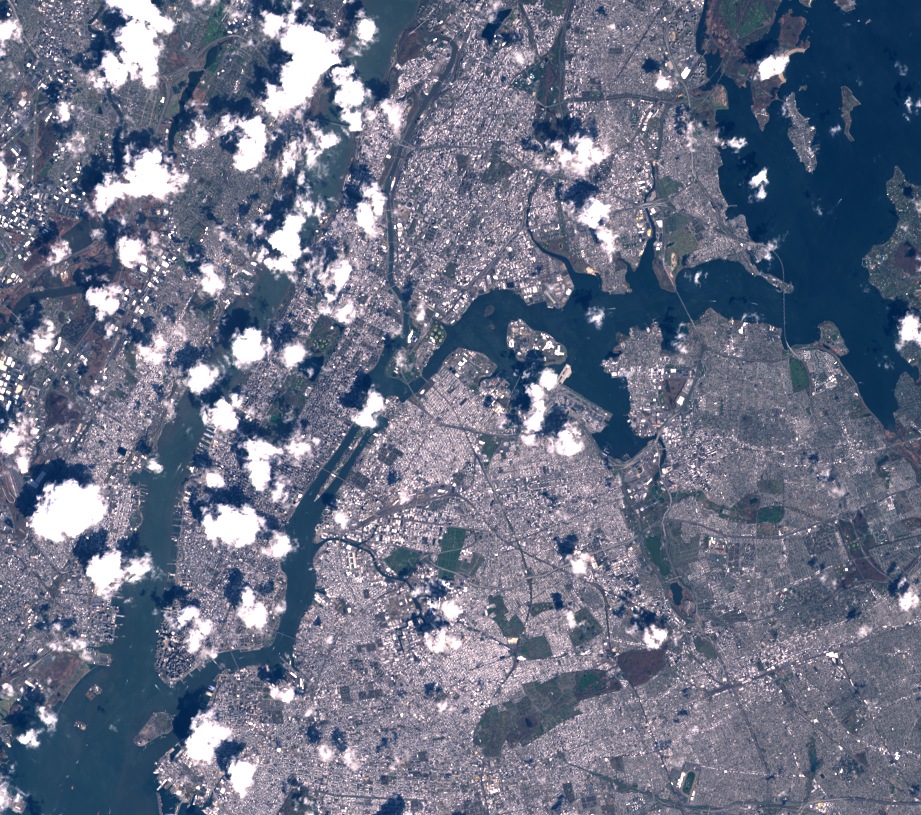
\includegraphics[width=1\textwidth]{figures/intro/landsat.png}
        \end{figure}
        \begin{enumerate}
            \item ImageJ\cite{schneiderNIHImageImageJ2012}, ImagePlot\cite{studiesCulturevisImageplot2021}\item Napari\cite{nicholas_sofroniew_2021_4533308}
        \end{enumerate}
        \pause
        \column{0.33\textwidth}
        \begin{figure}
            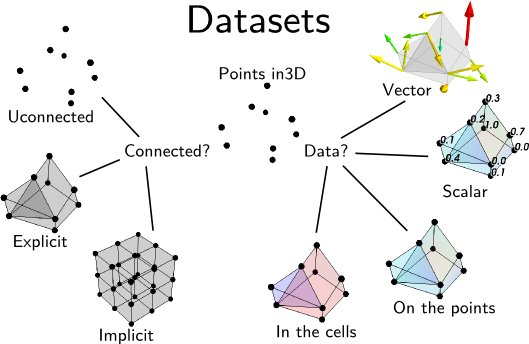
\includegraphics[width=1\textwidth]{figures/intro/dataset_diagram.png}
            \caption{Data Representation, MayaVi 4.7.2 docs\cite{DataRepresentationMayavi}}
        \end{figure}
        \begin{enumerate}
            \item Matplotlib\cite{hunterMatplotlib2DGraphics2007}, 
            \item VTK \cite{hanwellVisualizationToolkitVTK2015,geveci2012vtk}, MayaVi\cite{RamachandranMayaVI2011}, ParaView\cite{ahrens2005paraview}, Titan\cite{brianwylieUnifiedToolkitInformation2009}
        \end{enumerate}
    \end{columns}
\end{frame}

\begin{frame}{Structure is encoded in variables and continuity}
    \begin{figure}
        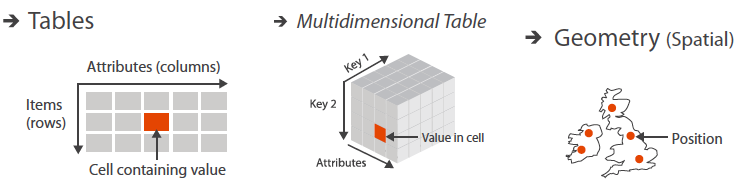
\includegraphics[width=1\textwidth]{figures/intro/munzner_datatypes.png}
        \caption{Image is figure 2.8 in Munzner's Visualization Analysis and Design\cite{munznerVisualizationAnalysisDesign2014}}
    \end{figure}
    \begin{description}
        \item[binding] metadata are structural \textit{keys} with associated \textit{values} (Munzner \cite{munznerVisualizationAnalysisDesign2014})] 
        \item[continuity] Fiber bundles can be a common data abstraction (Butler \cite{butlerVectorBundleClassesForm1992,butlerVisualizationModelBased1989})
        \item[variables] Fibers can hold schema like encodings of variables (Spivak \cite{spivakDatabasesAreCategories2010,spivakSIMPLICIALDATABASES})
    \end{description}
\end{frame}

\begin{frame}{Visualizations are (mostly) evaluated on equivariance}
    \begin{description}
        \item[Expressiveness] structure preserving mappings from data to graphic (Mackinlay \cite{mackinlayAutomatingDesignGraphical1986})
        \item[Effectiveness] design choices made in deference to perceptual saliency \cite (Mackinlay \cite{clevelandResearchStatisticalGraphics1987,clevelandGraphicalPerceptionTheory1984,chambersGraphicalMethodsData1983a, munznerVisualizationAnalysisDesign2014})
        \item[Naturalness] easier to understand when properties match (Norman \cite{norman_things_smart})
        \item[Graphical Integrity] graphs show \textbf{only} the data (Tufte \cite{tufteVisualDisplayQuantitative2001})
    \end{description}
\end{frame}


\begin{frame}{Models describe composition}
    \begin{description}
        \item[language model] APT: syntax and semantics of visualization (Mackinlay  \cite{mackinlayAutomatingDesignGraphical1986, mackinlayAUTOMATICDESIGNGRAPHICAL1987})
        \item[functional dependencies] constrained maps between data and visual representation(Sugibuchi \cite{sugibuchiFramwork2009}) 
        \item[category theory] the semiotics of visualization are commutative (Vickers \cite{vickersUnderstandingViz2013})
        \item[algebraic process] data ($\alpha$) and viz ($\omega$) transforms are symmetric (Kindlmann and Scheidegger \cite{kindlmannAlgebraicProcessVisualization2014})
        \begin{columns}
            \column{.5\textwidth}
       
            \begin{description}
                \item[D] data 
                \item[R] representations
                \item[V] visualizations
            \end{description}
            \column{.5\textwidth}
            \begin{equation*}
                \begin{tikzcd}[ampersand replacement=\&]
                    D \arrow[d, "\alpha"'] \arrow[r, "r_1"] \& R \arrow[r, "\nu"]  \& V \arrow[d, "\omega"] \\
                    D \arrow[r, "r_2"']                     \& R \arrow[r, "\nu"'] \& V                    
                \end{tikzcd}
                \end{equation*}
       
        \end{columns} 
     
    \end{description}
\end{frame}


\subsection{Contributions}
\begin{frame}{Contributions}
    \begin{description}
        \item[Topological] topology preserving relationship between data and graphic via continuous maps
        \item[Equivariant] property preservation from data component to visual representation as equivariant maps that carry a homomorphism of monoid actions
        \item[Artist] functional oriented visualization tool architecture built on the mathematical model to demonstrate the utility of the model
        \item [Model] prototype of the architecture built on Matplotlib's infrastructure to demonstrate the feasibility of the model
    \end{description}
\end{frame}

\section{Mathematical Framework}

\begin{frame}{Topological Equivariant Artist Model}
    The Artist $\mathscr{\vartist}$ is a map from data $\mathscr{\dtotal}$ to graphic $\mathscr{\gtotal}$
    \begin{equation}
        \mathscr{\vartist}: \mathscr{\dtotal} \rightarrow \mathscr{\gtotal}
    \end{equation}
    \pause
     that carries a homomorphism of monoid actions 
    \begin{equation}
    \varphi: \monoid \rightarrow \monoid^{\prime}
    \end{equation}
    \pause
    such that artists are equivariant maps 
    \begin{equation}
    \mathscr{\vartist}(m\cdot \delement) = \varphi(m)\cdot\mathscr{\vartist}(\delement) 
    \end{equation}
    \pause 
    with a deformation retraction from graphic to data space. 
    \note{some kinda words about the continuity}
\end{frame}

\subsection{Data Model}

\begin{frame}{Data Bundle}
    \begin{figure}
        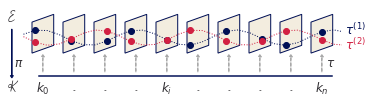
\includegraphics[width=1\textwidth]{figures/math/fiberbundle.png}
    \end{figure}
    A fiber bundle is a tuple $(\dtotal,\,\dbase,\,\pi ,\,\dfiber)$ defined by the projection map $\pi$
    \begin{equation}
        \label{eq:fiber_bundle}
        \begin{tikzcd}[ampersand replacement=\&]
            \dfiber \arrow[r, hook] \& \dtotal \arrow[r, "\pi"] \& \dbase
        \end{tikzcd}
    \end{equation}
    where \dtotal\ is the total data space, \dfiber\ is the variable space, and \dbase\ encodes the continuity.
\end{frame}

\begin{frame}{Variables: Fiber}
    Given a space of all possible values \ftotal\
    \begin{equation}
        \label{eq:data_types}
        \begin{tikzcd}[ampersand replacement=\&]
            \fttype \arrow[r] \arrow[d, "\pi_{\fsection}"'] \& \ftotal \arrow[d, "\pi"] \\
            \fnames \arrow[r, "\fsection"']                  \& \ftypes       
        \end{tikzcd}
    \end{equation}
    a fiber component is the restricted space $\ftotal_{\fsection(\fname)}$. 
    \begin{equation}
        \dfiber = \ftotal_{\fsection(\fname)} = \ftotal_{\ftype} 
    \end{equation}
    \begin{description}
        \item[\ftypes] data types of the variables in the dataset 
        \item[\ftotal] disjoint union of all values of type $\ftype \in \ftypes$ 
        \item[\fnames] variable names, $\fname \in \fnames$
        \item[\fttype] \ftotal\ restricted to the data type of a named variable   
    \end{description}
\end{frame}

\begin{frame}{Variable types are dimensions of the fiber}
    \begin{figure}[H]
        \begin{subfigure}{.49\textwidth}
            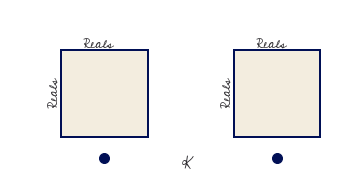
\includegraphics[width=\textwidth]{figures/math/temp_1k.png}
            \caption{}
            \label{fig:fiber_example_plane}
        \end{subfigure}
        \begin{subfigure}{.49\textwidth}
            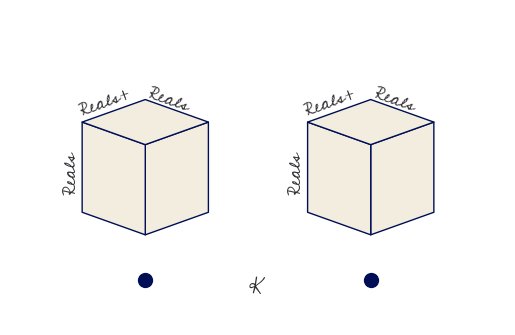
\includegraphics[width=\textwidth]{figures/math/temp_3f.png}
            \caption{}
            \label{fig:fiber_example_cube}
        \end{subfigure}
        \caption{}
        \label{fig:data_fiber_example}
    \end{figure}
    \begin{description}
        \item[\ref{fig:fiber_example_plane}]  $\dfiber=\reals\times\reals$, (time, temperature)
        \item[\ref{fig:fiber_example_cube}]  $\reals\times\realsp\times\reals$, (time, wind=(speed, direction))
    \end{description}
\end{frame}


\begin{frame}{Structure of Components: Monoid \& Monoid Actions}
A monoid \monoid\ is a set with
\begin{description}
    \item[associative binary operator] $\ast:\monoid \times \monoid\rightarrow \monoid$
    \item[identity element] $e\in \monoid$ such that $e\ast a= a \ast e = a$ for all $a \in \monoid$. 
\end{description}
\pause
\begin{block}{left monoid action}
A set \dfiber\ with an action $\bullet: \monoid\times \dfiber \rightarrow \dfiber$ with the properties:
    \begin{align*}
        \textbf{associativity}\;& \text{for all } f,g \in \monoid \text{ and } x\in \dfiber,\, f\bullet(g\bullet x) = (f\ast g) \bullet x\\
        \textbf{identity}\;& \text{for all } x\in \dfiber, e\in \monoid,\,  e\bullet x = x 
    \end{align*}
\end{block}
\end{frame}

\begin{frame}{Monoid Actions: Permutation}
    \begin{figure}
        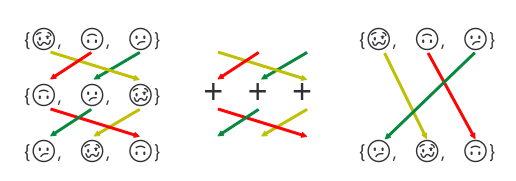
\includegraphics[width=1\linewidth]{figures/math/monoid_emoji.png}
    \end{figure}
\end{frame}

\begin{frame}{Why monoids? partial orders}
    \begin{figure}
        \begin{overprint}
            \onslide<1|handout:0>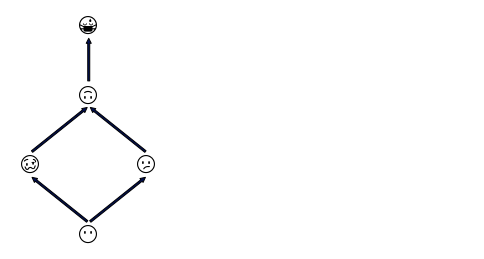
\includegraphics[width=1\linewidth]{figures/math/monoid_hasse.png}
            \onslide<2|handout:0>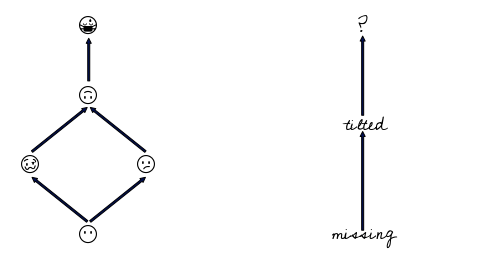
\includegraphics[width=1\linewidth]{figures/math/monoid_monotone.png}
            \onslide<3>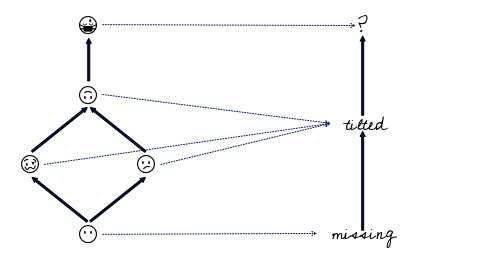
\includegraphics[width=1\linewidth]{figures/math/monoid_maps.png}
        \end{overprint}
    \caption{Inspired by definition 1.59 diagram in Spivak and Fong's An Invitation to Applied Category Theory \cite{fongInvitationAppliedCategory2019}}
    \end{figure}
\end{frame}

\begin{frame}{Data Continuity: Base space}
    \begin{figure}[H]
    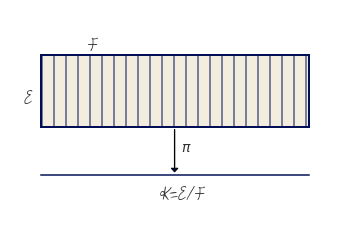
\includegraphics[height=.5\textheight]{figures/math/k_qspace.png}
    \label{fig:base_space_div}
\end{figure}
where the total space can be decomposed into components 
\begin{equation}
    \pi:\dtotal_1\oplus\ldots\oplus \dtotal_i \oplus\ldots \oplus \dtotal_n \rightarrow \dbase
\end{equation}
\end{frame}

\begin{frame}{Data connectivity is encoded as the base space}
    \begin{figure}[H]
        \begin{subfigure}{.49\textwidth}
            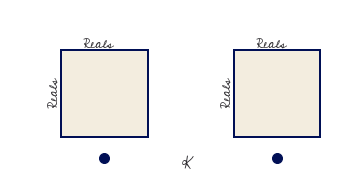
\includegraphics[width=\textwidth]{figures/math/temp_1k.png}
            \caption{}
            \label{fig:base_example_discrete}
        \end{subfigure}
        \begin{subfigure}{.49\textwidth}
            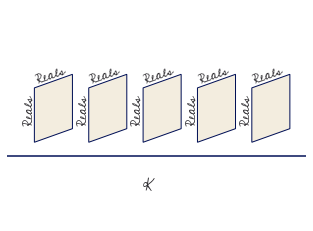
\includegraphics[width=\textwidth]{figures/math/temp_2f.png}
            \caption{}
            \label{fig:base_example_continuous}
        \end{subfigure}
        \caption{}
        \label{fig:base_example}
    \end{figure}
    \begin{description}
        \item[\ref{fig:base_example_discrete}] data is discrete 0D points
        \item[\ref{fig:base_example_continuous}]  data is lies on the 1D continuous interval \dbase\
    \end{description}
\end{frame}

\begin{frame}{Values: Section}
    For any fiber bundle, there exists a map
    \begin{equation}
        \begin{tikzcd}[ampersand replacement=\&]
            \dfiber \arrow[r, hook] \& \dtotal \arrow[d, "\pi"'] \\
                              \& \dbase \arrow[u, "\dsection"', bend right]
        \end{tikzcd}
    \end{equation}
     s.t. $\pi(\dsection(\dbasepoint)) = \dbasepoint$.  Set of all global sections is denoted $\Gamma(\dtotal)$.
     \pause
     \begin{block}{Record}
     Assuming a trivial fiber bundle $\dtotal = \dbase \times \dfiber$, the section is 
\begin{equation}
    \label{eq:section_return}
    \dsection(\dbasepoint) = (\dbasepoint, (g_{\dfiber_{0}}(\dbasepoint), \ldots, g_{\dfiber_{n}}(\dbasepoint)))
\end{equation}
where $g: \dbase \rightarrow \dfiber$ is the index function into the fiber.
\end{block}
\end{frame}

\begin{frame}{Sample dataset}
    \begin{figure}[H]
        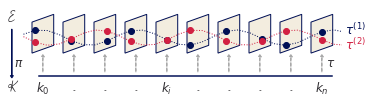
\includegraphics[width=1\linewidth]{figures/math/fiberbundle.png}
        \label{fig:data_sections}
    \end{figure}
    \begin{itemize}
        \item \dfiber\ is $\reals\times\reals$
        \item \dbase\ is interval $\left[0,1\right]$
        \item $\dsection^{(1)}$ is a $sin$ function
        \item $\dsection^{(2)}$ is a $cos$ function
        \item $\dsection^{(1)}, \dsection^{(2)} \in \Gamma(\dtotal)$
    \end{itemize}
  
\end{frame}

\subsection{Graphics}
\begin{frame}{Graphic Bundle}
    The graphics bundle is a tuple $(\gtotal,\,\gbase,\,\pi ,\,\gfiber)$ defined by the projection map $\pi$
    \begin{equation}
        \begin{tikzcd}[ampersand replacement=\&]
            \gfiber \arrow[r, hook] \& \gtotal \arrow[d, "\pi"'] \\
                              \& \gbase \arrow[u, "\gsection"', bend right]
        \end{tikzcd}
    \end{equation}
    where \gsection\ is the fully encoded graphic. 
    \pause
    \begin{block}{Example: 2D opaque image}
    The target display is $\gfiber=\reals^5$ with elements 
    \begin{equation*}
    (x,\, y,\, r,\, g,\, b) \in \gfiber
    \end{equation*}
    returned by \gsection\ such that a graphic has color and 2D position.
    \end{block}

\end{frame}
\begin{frame}{Graphic Continuity}
    The surjective map $\vindex: \gbase \rightarrow \dbase$
    \begin{equation}
        \begin{tikzcd}[ampersand replacement=\&]
            \dtotal \arrow[d, "\pi"'] \& \gtotal \arrow[d, "\pi"'] \\
            \dbase                   \& \gbase \arrow[l, "\vindex"']
        \end{tikzcd}
    \end{equation}
    goes from region $\gbasepoint \in \gbase_{\dbasepoint}$ to its associated point $\dbasepoint$ in data space. 
\pause
    \begin{figure}[H]
        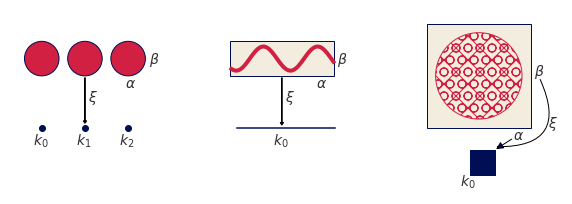
\includegraphics[width=1\textwidth]{figures/math/retraction_maps.png}
        \label{fig:graphic_retraction_map}
    \end{figure}
\end{frame}

\subsection{Artist}
\begin{frame}{Topological Equivariant Artist Model}
The topological artist \vartist\ is a monoid equivariant sheaf map 
\begin{equation}
    \label{eq:artist_diagram}
    \begin{tikzcd}[ampersand replacement=\&]
        \dtotal^{\prime} \arrow[r, "\vchannel"] \arrow[rd, "\pi"'] \& \vtotal \arrow[d, "\pi"] \& \vindex^*\vtotal \arrow[r, "\vmark"] \arrow[d, "\vindex^*\pi"'] \arrow[l, "\vindex^*"'] \& \gtotal \arrow[ld, "\pi"] \\
                                              \& \dbase                  \& \gbase \arrow[l, "\vindex"']                                              \&                    
        \end{tikzcd}
\end{equation}

where the artist $\vartist: \mathcal{O}(\dtotal) \rightarrow \mathcal{O}(\gtotal)$ takes as input $\dtotal^{\prime}=\mathcal{J}^{2}(\dtotal)$. 
\end{frame}

\begin{frame}{Visual Bundle}
    The visual bundle is a tuple $(\vtotal,\,\dbase,\,\pi ,\,\vfiber)$ defined by the projection map $\pi$
    \begin{equation}
        \begin{tikzcd}[ampersand replacement=\&]
            \vfiber \arrow[r, hook] \& \vtotal \arrow[d, "\pi"'] \\
                              \& \dbase \arrow[u, "\vsection"', bend right]
        \end{tikzcd}
    \end{equation}
    where \vsection\ is the visual variable encoding\cite{bertinIIPropertiesGraphic2011} of the representation of the data section \dsection. 
    \begin{block}{Example: position and color}
        Given an artist with parameters $\{xpos, ypos, color\}$, a sample visual section \vsection\ could be $\{.5, .5, (255, 20,147)\}$
    \end{block}
\end{frame}

\begin{frame}{Visual Channel Encoders}
We define the visual transformers \vchannel\ on components of the data bundle $\dsection_{i}$
\begin{equation}
    \label{eq:nu_expanded}
    \{\vchannel_{0}, \ldots, \vchannel_{n}\}: \{\dsection_{0}, \ldots, \dsection_{n}\} \mapsto \{\vsection_{0}, \ldots, \vsection_{n}\}
\end{equation}
as the set of equivariant maps with the constraint 
\begin{equation}
    \vchannel_i(m_{\delement}(\dtotal_i)) = \varphi(m_{\delement})(\vchannel_i(\dtotal_i))
\end{equation} 
where $\varphi:\monoid\rightarrow \monoid^{\prime}$ carries a homomorphism of monoid actions. 
\end{frame}

\begin{frame}{Example: Nominal Equivariance}
    \begin{figure}
        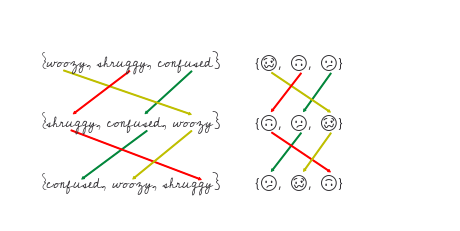
\includegraphics[width=1\textwidth]{figures/math/equivariance_nu.png}
        \caption{The actions on the text data are the same as the actions on the visual representation of that data as emojis.}
    \end{figure}
\end{frame}

\begin{frame}{Visualization Assembly Function}
    \begin{figure}
        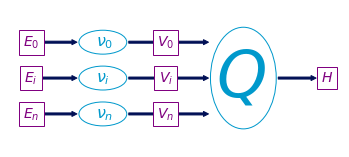
\includegraphics[width=\textwidth]{figures/math/path_of_q.png}
    \end{figure}
\end{frame}

\begin{frame}{Glyph}
    The glyph is the graphic generated by $\vmark(\gbase_{\dbasepathpoint})$ where the path connected components $\dbasepath \subset \dbase$ are defined 
    \begin{equation}
    \dbasepath = \{\dbasepathpoint \in \dbase \text{ s. t. } \exists \gamma \text{ s.t. } \gamma(0)=\dbasepoint \text{ and }\gamma(1)=\dbasepathpoint\}
    \end{equation}
    such that the  path $\gamma$ from \dbasepoint\ to \dbasepathpoint\ is a continuous function from the interval [0,1] and $\gbase_{\dbasepathpoint}$ is the region
    \begin{equation}
        \begin{tikzcd}[ampersand replacement=\&]
            \gtotal \arrow[r, shift left] \& \gbase_\dbasepathpoint \arrow[rr, "\vindex(\gbasepoint)", shift left] \arrow[l, "\gsection(\gbase_\dbasepathpoint)"] \& \& \dbasepath_{\dbasepoint} \arrow[ll, "\vindex^{-1}(\dbasepath)"]
            \end{tikzcd}
        \label{eq:mark}
    \end{equation}
    such that the glyph is differentiable, in keeping with Ziemkiewicz and Kosara's description of a glyph\cite{ziemkiewiczEmbeddingInformationVisualization2009}.
\end{frame}

\begin{frame}{Visualization Equivariance}
    If \vmark\ is applied to $\vsection, \vsection^{\prime}$ that generate the same \gsection\, 
    \begin{equation}
    \vmark(\vsection) = \vmark(\vsection^{\prime})\implies \vmark(m\circ\vsection) = \vmark(m\circ\vsection^{\prime})
    \end{equation}
    then the output of both sections acted on by the same monoid $m$ must be the same. 
    \pause
    \begin{figure}[H]
        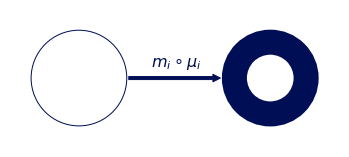
\includegraphics[width=\textwidth]{figures/math/diff_type_q.png}
    \end{figure}
\end{frame}

\begin{frame}{Scatter: $\vmark(xpos, ypos)(\alpha, \beta)$}
    \begin{figure}[H]
        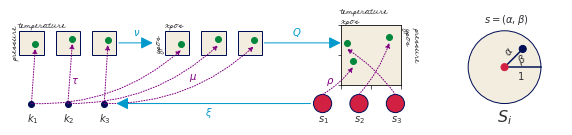
\includegraphics[width=1\textwidth]{figures/math/scatter.png}
    \end{figure}
    
    \begin{align*}
        x &= size *\alpha \cos(\beta) + xpos \\
        y &= size *\alpha \sin(\beta) + ypos
    \end{align*}    
\end{frame}

\begin{frame}{Line: $\vmark(xpos, \hat{n_{1}}, ypos, \hat{n_{2}})(\alpha, \beta)$ }
    \begin{figure}[H]
        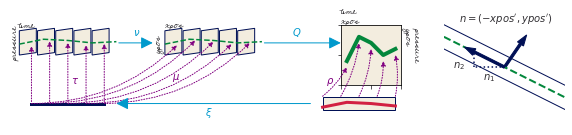
\includegraphics[width=1\textwidth]{figures/math/line.png}
    \end{figure}
        \begin{equation*}
            \lvert n \rvert = \sqrt{{n_{1}}^2 + {n_{2}}^2},\; 
            \hat{n_{1}} = \frac{n_1}{\lvert n \rvert}, \; \hat{n_{2}} = \frac{n_2}{\lvert n \rvert}
        \end{equation*}
    \begin{align*}
     x = xpos(\vindex(\alpha)) &+ width*\beta\hat{n_1}(\vindex(\alpha)) \\
     y = ypos(\vindex(\alpha)) &+ width*\beta\hat{n_2}(\vindex(\alpha)) 
    \end{align*}
\end{frame}

\begin{frame}{Image $\vmark(xpos, yposcolor)$}
    \begin{figure}[H]
        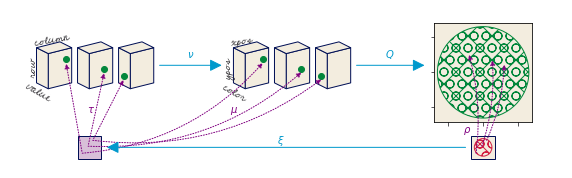
\includegraphics[width=1\textwidth]{figures/math/image.png}
    \end{figure}
    \begin{align*}
        R &= R(\vindex(\alpha, \beta))\\
        G &= G(\vindex(\alpha, \beta))\\
        B &= B(\vindex(\alpha, \beta))
    \end{align*}
\end{frame}


\section{References}
\begin{frame}[allowframebreaks]{References}
%\printbibliography
\end{frame}
\appendix 
\begin{frame}{Rendering: Define a Pixel}
    \begin{columns}
        \column{0.5\textwidth}
        Given a pixel
        \begin{equation}
        p=\left[y_{top}, y_{bottom}, x_{right}, x_{left}\right]
        \end{equation}
        the inverse map of the bounding box 
        \begin{equation}
        \gbase_{p} ={\gsection_{xy}}^{-1}(p)
        \end{equation}
        is a region $\gbase_p \subset \gbase$ such that 
        \begin{align}
            \scriptstyle r_p &= \scriptstyle \iint\limits_{S_p} \rho_r(s)ds^{2}\\
            \scriptstyle g_p &= \scriptstyle \iint\limits_{S_p} \rho_g(s)ds^{2}\\
            \scriptstyle  b_p &= \scriptstyle \iint\limits_{S_p} \rho_b(s)ds^{2}
        \end{align}
        yields the color of the pixel. 
        \column{0.5\textwidth}
        \begin{figure}[H]
            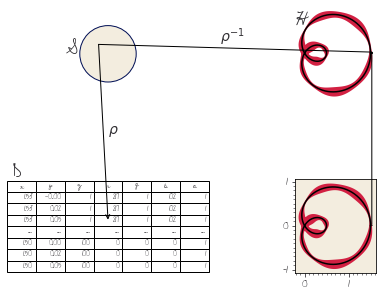
\includegraphics[width=\textwidth]{figures/math/render.png}
        \end{figure}
    \end{columns}
\end{frame}


\end{document}

